
\section*{Abstract}

Wastewater-based epidemiology has long been proposed as a tool for population health monitoring, with applications ranging from infectious disease surveillance to drug consumption estimation. To date, however, there are few examples of wastewater epidemiology being implemented in practice. Here, we propose a novel platform that adapts existing wastewater-based epidemiology approaches for community-level public health surveillance. We integrate sewage network and population information to identify a sampling manhole representative of a residential community and show that the wastewater sampled at this upstream manhole contains more human-derived bacteria and metabolites than downstream wastewater treatment plant samples, which are the usual sampling locations in wastewater epidemiology. Our method to perform untargeted metabolomics on raw sewage allows for the identification of multiple glucuronide compounds, which are indicative of direct human excretion and typically too unstable to be detected in wastewater. We show that these compounds are absent in downstream samples, but abundant in our residential sewage samples. Next, we perform an hourly 24-hour sampling campaign to identify human and environmental components of the sewage metabolome and microbiome based on diurnal variations. We confirm urinary and fecal metabolites and find that their dynamics reflect human behavior but differ from each other. Finally, we propose that mining untargeted data derived from residential sewage opens additional possibilities for identifying biomarkers with direct public health or policy relevance and show preliminary results from the metabolomics data. Together, these results suggest a novel approach for implementing wastewater epidemiology in urban settings that provides a new source of community-level health data and which could be developed into a citywide public health observatory.

\section{Introduction}

Urbanization is a globally increasing phenomenon. By 2050, 70\% of the world's population will live in cities where 80% of the global GDP will be generated. Cities are thus prime locations to deliver services that improve the wellbeing of residents. However, public health officials in cities tend to operate under financial constraints and with limited data to establish priorities and measure the impact of their programs. Wastewater has been proposed as a source of data on population health and behavior that can fill this gap at relatively low cost for public health officials \cite{Daughton2018}.

Wastewater-based epidemiology could have enormous benefit to public health practice, providing real-time assessment of population health and generating data to support public health and city policies. Currently, most public health surveillance is based on reports from hospitals and other clinical centers, and appropriate responses are initiated after enough clinical cases have been reported. Wastewater-based public health surveillance platforms, in contrast, could provide real-time data on emerging outbreaks before a critical mass of patients have gotten sick \cite{Manor2014,Hellmer2014}. Viral and bacterial pathogens shed in stool could be directly detected in sewage, triggering the deployment of coordinated awareness campaigns or other public health interventions to areas with the largest number of sick patients, all without needing to wait for case reports from hospitals. In addition to identifying emerging outbreaks, wastewater could provide a novel source of data to evaluate the effectiveness of policies intended to have long-term effects on a population's health \cite{Daughton2018}. For example, rather than waiting years to measure the impact of taxing sugary drinks on population obesity levels, biomarkers of obesity or consumption could be directly measured in sewage before and after the policy roll-out, thus providing a more immediate measure of the impact of policy on targeted outcomes.

Wastewater-based epidemiology has been proposed for many exciting applications. It has been shown to be useful as an early indicator of poliovirus outbreaks to target vaccination campaigns in polio-free countries \cite{Manor2014,Kaliner2015} and to quantify asymptomatic circulation \cite{Berchenko2017}. Environmental surveillance of typhoid and antimicrobial resistance through urban wastewater are emerging areas of interest in global and public health organizations \cite{Pehrsson2016,Initiatives2018}. Besides infectious disease, methods have been developed and standardized over the last decade to successfully provide continuous data on illicit drug consumption at the national- and regional-level in Australia \cite{AustralianReport} and over 60 European cities and towns \cite{vanNuijs2018,Thomas2012,BazLomba2016}. The academic community is now interested in branching out to measure lifestyle chemicals and biomarkers of health such as obesity levels \cite{Daughton2018,Arnaud2018,Newton2015}. More recently, wastewater testing has been proposed as a promising tool to tackle the opioid epidemic that is severely affecting the U.S \cite{Keshaviah2016,Keshaviah2017}. However, apart from successful poliovirus surveillance and, to a lesser extent, national-level drug consumption surveillance programs, most application areas remain proof-of-concept academic projects and have yet to be implemented into public health and other public service delivery agencies.

Despite great technical advances over the past decades, wastewater testing still presents considerable challenges that decrease its usefulness to public health officials and policy-makers. In most proposed applications, wastewater is sampled at downstream sites like pump stations or treatment plants \cite{Manor2014,Hellmer2014}. While downstream collection sites are easily accessible and cost-effective, they impose barriers to data interpretation in the public health context. Wastewater at treatment plants is a combination of residential households and commercial and industrial buildings, and it may represent one or more municipalities. These factors create technical biases in the data and prevent clear consumption or infection rates from being calculated from measured quantities. Additionally, if the interest is to compare several cities, collection from different wastewater treatment plants or other downstream sites may introduce confounding factors, such as representation of different population sizes \cite{OBrien2013}, large variation in wastewater travel time from different sources, different rates of in-sewer degradation of chemical \cite{Thai2014} and bacterial biomarkers, and collection with ad-hoc sampling equipment that prevents researchers from optimizing collection parameters to obtain representative samples \cite{Ort2010}. Finally, while collecting composite samples from wastewater treatment plants (WWTPs) is practical and cost-effective to generate national estimates \cite{Zuccato2008,Castiglioni2006,Thomas2012}, data from WWTPs is not optimal for city officials since it lacks geographic specificity. Finally, public health officials are interested in a broad range of human health biomarkers but it is not straightforward to know what markers are stable and quantifiable in wastewater collected from different regions \cite{Arnaud2018}.

Here, we propose a novel implementation of wastewater epidemiology that addresses these challenges and develops wastewater testing as a platform to directly measure the health of urban communities and facilitate applications to public health. We combine demographic, sewage, and geographic data sources to curate and select an upstream sampling site that reflects a residential population. By mining untargeted microbiome and metabolomics data, we show that residential sewage reflects human diurnal activity and identify human-derived biomarkers which can be specifically separated from environmental contributors. Together, this work is the first to show that upstream wastewater sampling could provide a novel useful data source for public health agencies.

\section{Results}

\subsection{Upstream residential catchments provide more useful public health information than WWTP samples}

Integrating GIS datasets with demographic and sewage network information enables the selection of sampling sites with carefully curated technical and population characteristics. We defined residential catchments as those which represent areas with at least 80\% residential land use, a population of over 5,000 people, and a maximum sewage travel time of less than 60 minutes (Fig. \ref{24hr:fig1}A). We screened all manholes in our municipality and selected a manhole which met these criteria (Fig. \ref{24hr:fig1}A). From a usability perspective, data from residential catchments will be more actionable by municipal public health departments because sites can be selected to mostly capture resident rather than transient populations, and to have the spatial resolution that matches their public health interventions.

Besides providing geographical specificity to the sample, residential catchments mitigate variability in population size and sewage travel time observed at WWTPs. Our selection criteria produces catchments with similar population sizes by design (5,000--10,000 inhabitants) rather than the large range observed (1,000--2,000,000 inhabitants) in WWTPs (Supp. Fig. \ref{24hr:figS1}, \cite{Newton2015}). Additionally, residential catchments are more likely to contain even representation of all households in the catchment compared to WWTPs: in our residential catchment, sewage from every source travels at most 45 minutes to the sampling point and the distribution of travel times is narrowly-distributed (Fig. \ref{24hr:fig1}A). Sewage at WWTPs, on the other hand, can have travelled anywhere from minutes to hours before it reaches the sampling point. Sampling in residential catchments therefore mitigates the need to correct for unequal population sizes and travel times to some extent.

Residential sewage contains more direct chemical markers of human consumption and behavior than sewage sampled at WWTPs. We sampled a residential sewer (selected as described above) and a downstream pump station (Fig. \ref{24hr:fig1}B) and performed untargeted metabolomics and 16S rRNA sequencing on the filtrate and bacterial cells, respectively. 34.5\% of the metabolites detected in both sewer and WWTP samples (n=245/710) had significantly different concentrations (p-value $<$ 0.05 independent T-test with FDR correction for multiple testing). Of these differentially abundant metabolites, 73\% (n=179/245) decreased or disappeared completely from wastewater collected at the WWTP, including many metabolites from human activity as defined later in this paper (Fig. \ref{24hr:fig2}A yellow dots, Fig. \ref{24hr:fig3}B yellow bars, Supp. Fig. \ref{24hr:figS2} cluster M1). Similarly, we found that residential sewage contained a higher proportion of human-associated bacteria than WWTP sewage. On average, 66\% of the microbial community from residential sewage was of human fecal origin, compared to 51\% in the pump station samples (Fig. \ref{24hr:fig2}B), with the Ruminococcaceae, Lachnospiraceae, Prevotellaceae, Veillonellaceae and Erysipelotrichaceae families being reduced (Supp. Fig. \ref{24hr:figS3}). These results are similar to those reported in Newton et al. \cite{Newton2015}, where on average 15\% of sequences in WWTP sewage had human fecal origin. Together, these results indicate that wastewater from residential catchments which has been traveling in sewers for less than one hour contains many human biomarkers that are absent in wastewater collected at WWTPs.

Furthermore, performing untargeted metabolomics on residential catchment samples extends the possible biomarkers that can be monitored through wastewater epidemiology. We identified 22 glucuronide compounds in our untargeted data (see Methods). Glucuronides are chemical groups added to exogenous molecules by the human liver to aid in their excretion and are thus indicators of human excretion, distinguishing between molecules simply discarded into the sewers versus those consumed and excreted by humans and providing direct evidence of consumption. However, many bacteria carry glucuronidase enzymes that release the glucuronide group to use as carbon source \cite{Pollet2017}, and these unstable molecules have previously been difficult to identify in sewage samples from WWTPs \cite{Jacox2017}. In our data, the majority of the identified glucuronides were significantly reduced or altogether absent in wastewater collected at the WWTP (Figure \ref{24hr:fig2}C). Sampling upstream allows for the detection of these unstable molecules and also more generally expands the number of compounds which can be measured. Molecules which are usually difficult to measure by mass spectrometry in wastewater because they do not ionize well should be captured in residential catchments, since the human body excretes compounds by dissolving them in urine or stool and therefore naturally converts exogenous compounds into more ionizable chemical forms. Thus, detecting a large number of glucuronides in our residential catchment sewage sample suggests that expanding wastewater monitoring to chemical variants of molecules of interest may be beneficial for future environmental surveillance applications.

\subsection{Residential sewage microbiome and metabolome contain both human- and environmentally-derived components}

Chemical and bacterial biomarkers detected in residential sewage reflect the daily timescale of human activity. We used the average sewage flow rate over two months as a proxy for human activity (Figure \ref{24hr:fig3}). We hypothesized that human-associated metabolites and bacteria would increase during the day, when the contributing population would be more active, and decrease at night. We collected hourly samples over 24 hours from the residential catchment manhole and produced 16S rDNA sequencing and untargeted metabolomics profiles (Figure \ref{24hr:fig3}A). We co-clustered metabolomic features (n=3,672) and microbial OTUs (n=254) based on their Spearman correlation (Fig. \ref{24hr:fig3}B \& D, Supp. Fig. \ref{24hr:figS2}), and found that the metabolic features grouped into two main clusters (M1 and M2), while bacterial OTUs produced three groups (O1 and O2 are highlighted). The M1 metabolite cluster (n=2,815) had strong positive correlation with the O1 bacterial cluster (n=41) and negative correlation to the O2 bacterial cluster (n=84). The majority of metabolites and bacteria in these groups also correlated with the average flow rate in the sewer, increasing during the day and becoming drastically less abundant at night (Fig. \ref{24hr:fig3}B \& D).

Metabolites and bacteria in sewage separate into human and environmental contributions. Groups M1 and O1 were enriched in human-derived bacteria and metabolites, while groups M2 and O2 contained bacteria and metabolites derived from the environment (Fig. \ref{24hr:fig3}C). The cluster M1 was statistically enriched in matches to human metabolites compared to the M2 cluster (Fig. \ref{24hr:fig3}C), and includes known urinary and fecal metabolites. Twenty-two metabolic features in M1 were identified as glucuronide compounds of hormones, bile acids and pharmaceuticals, which are direct markers of human excretion as discussed above. Bacteria in the cluster O1 were putatively identified as coming from human gut microbiomes. Cluster O1 included 41 bacterial OTUs primarily from the Firmicutes and Bacteroidetes phyla, which are major components of the human gut flora (Fig. \ref{24hr:fig3}D). Additionally, the top 10 most abundant bacterial families in human stool (Human Microbiome Project) made up 65\% of the community in the O1 group (Supp. Fig. \ref{24hr:figS4}). Similar to what was observed in the metabolites, O1 bacteria had a dip in relative abundance during nighttime (Figure \ref{24hr:fig3}B). Clusters M2 and O2, on the other hand, remained relatively constant through the day and likely reflect bacteria and metabolites sourced from environmental background rather than human activity. Cluster M2 had few putative human-associated hits, and had constant abundance through the day and nighttime. The molecules in this group likely represent chemicals derived from the environment or sewer biochemistry. Human-associated bacteria were similarly decreased in cluster O2: most of the OTUs were Proteobacteria, which are not major members of the normal gut flora, and human fecal bacterial families comprised only 1.4\% of the abundance of this cluster (Supp. Fig. \ref{24hr:figS4}). The relative abundance of cluster O2 increased at night, reflecting that these environmental made up a larger proportion of the residential sewage microbiome during periods of low human activity (Fig. \ref{24hr:fig3}D).

\subsection{Identification of potential public health biomarkers in residential sewage}

Urine and fecal contributions to residential sewage can be identified through untargeted analyses. We identified and confirmed metabolites corresponding to human urinary and fecal markers through a combination of MS2 matching and confirming with analytical standards. In our attempts to annotate metabolite features, we prioritized features with high abundance across all samples and in a few samples of interest (i.e. 8 am and 2 pm samples, which contained more metabolites and which we expected to correlate with human behavior). We screened the top mz values against METLIN and HMDB databases to find putative human-derived metabolites \cite{Wishart2012,Smith2005}. We confirmed features which putatively matched urinary or fecal markers and for which we could acquire analytical standards. Furthermore, we compared the MS2 fragmentation patterns for potential glucuronide compounds with their expected fragmentations and used diagnostic mz peaks to putatively confirm these compounds (see Methods). The most abundant feature in our dataset was confirmed via analytical standard as alpha-N-phenylacetyl-L-glutamine (PAG), a metabolite of phenylacetic acid and an end product of phenylalanine metabolism excreted in urine \cite{Seakins1971,Stein1954}. Previous studies on human physiology have found that PAG excretion remains constant in response to diet and does not exhibit diurnal cycling in individual patients \cite{Seakins1971}. Thus, the abundance of PAG in our sample likely correlates with the total volume of urine in sewage at any given time. Urobilinogen, a breakdown product of hemoglobin excreted primarily in stool \cite{Balikov1957}, was also confirmed via analytical standard. We also confirmed 4 bile acids (chenodeoxycholic acid, cholic acid, glycocholic acid, taurocholic acid), which represent the major primary conjugated and unconjugated bile acids produced by the liver to aid in digestion and which we considered as putative fecal markers.

The urinary and fecal metabolites reflected general diurnal human dynamics, but differed from each other (Figure \ref{24hr:fig4}). Both types of metabolites decreased at night, with the fecal markers almost completely disappearing while the urinary marker remained detectable. Fecal markers also showed significant spikes in the 8 am and 3 pm samples, and were slightly elevated throughout the evening (8 - 10 pm). The urinary marker, on the other hand, increased in the morning and stayed relatively consistent throughout the day. These patterns correspond with known patterns of human behavior: at night, people are less likely to wake up to defecate but do wake up to urinate. During the day, urination remains relatively constant across the entire population, but defecation probably spikes in the morning right after waking up and after meal times.

Furthermore, the daily dynamics of bile acids in residential sewage may reflect population-level behavior and physiology. During the day, levels of unconjugated cholic and chenodeoxycholic acids remained relatively constant but conjugated cholic acids (glycocholic and taurocholic acid) spiked after mealtimes (Fig. \ref{24hr:fig4}). In individuals, the liver synthesizes more bile acids from cholesterol after it is ingested during a meal \cite{Hofmann1989}. Levels of taurocholic acid are also known to increase significantly after meals, since the diet is the primary source of taurine in humans. The liver secretes only the conjugated forms of cholic acid, glycocholic and taurocholic acid, into the gut. Thus, the post-meal spikes in conjugated bile acids in our data may reflect not only more stool in the sewage but also an aggregate population-level increase in physiological production of bile acids by the liver in response to meals. The daily dynamics of fecal bile acid excretion has not been studied in humans, in part because it is difficult to access finely temporally-resolved data given that humans defecate only 1-3 times per day on average. These data suggest that analyzing physically aggregated biological data could provide another avenue by which to study human physiology or measure its functioning.

However, an alternative explanation for these spikes in conjugated bile acids may be that they reflect only incidental increases in the sampling of individuals with diarrhea at these times. Diarrhea is characterized by a decrease in the conversion of conjugated primary bile acids to their unconjugated forms. Furthermore, because our metabolomics data is generated from the liquid phase of wastewater after removing solids, diarrhea will contribute relatively more than solid stools to the sampled metabolites at any given time. Thus, our results are consistent with a sampling enriched in individuals with diarrhea at times when they defecate. By contrast, the contribution of stools from healthy individuals (as indicated by the levels of cholate and deoxcholate) remains relatively constant over the course of the day. Taken together, the findings that fecal and urinary metabolites differ in their dynamics and that individual people may disproportionately contribute to individual samples, suggest that developing methods to correct for biases in sampling and normalize for the number of people contributing to a given sample will be required before these data can be acted upon in public health contexts.

\section{Discussion}

The platform that we present is the first to adapt the practices of wastewater-based epidemiology specifically for the needs of city-level public officials, and is the first to leverage untargeted multi-omics data to examine the breadth of human biomarkers available in residential wastewater. Through high-throughput microbiome and metabolome analyses, we show that wastewater from residential catchments is a closer reflection of human health than wastewater collected at downstream sites. Wastewater from residential catchments contains more human metabolites and human-associated bacteria than wastewater from downstream sites, including unstable glucuronides which can be used as direct markers of human consumption. Untargeted analyses can identify glucuronides and potentially other chemical variants of molecules, expanding the scope of compounds amenable to wastewater surveillance. Moreover, metabolites and bacteria in residential sewage can be compartmentalized into human and environmental contributions, and human-associated components reflect known human behavior and activity. Finally, our data suggests that identifying biomarkers across many realms of interest such as human behavior, consumption, and health, may be possible through residential wastewater surveillance. However, incorporating residential sewage monitoring into public health departments will require addressing additional analytical, engineering, logistical, and ethical challenges.

First, models to estimate the population size contributing to a given sample will need to be developed in order to convert measured quantities into per capita rates. Samples taken from wastewater treatment plants can be reasonably expected to represent a large portion of the catchment population, representing thousands to hundreds of thousands of individuals. In contrast, the number of people represented in a residential sewage sample may fluctuate significantly in these smaller residential catchments. Without knowing how many people contributed to a given sample, it is not possible to interpret the quantities measured in a given sample: did one person excrete a large amount of the measured component, or did many people excrete a small amount of it? Knowing the``denominator'' of what is measured in sewage will be required to translate measured quantities into values that city officials can act on.

Scaling this work to the city-level will also require the development of new sampling equipment sampling campaign designs. Sampling equipment could be developed to aggregate flow-proportional samples over a full day, and more complex samplers could also perform some pre-processing or basic measurements \textit{in situ}. The sampling sites chosen in a given campaign could be optimized for a variety of purpose: covering as much of the population with the least number of sites, identifying hot spots where potential outbreaks are likely to begin, comparing neighborhoods with different socioeconomic characteristics or health behaviors, or standardizing sampling site characteristics to enable multi-city comparisons. Each of these approaches will have benefits and trade-offs, but all should be developed in partnership with city officials and community leaders to ensure public accountability, transparency, and ultimate benefit to the community.

Finally, data privacy and ethics should be considered in all stages of development and deployment. Sewage is a physical aggregate of multiple individuals, and so does not share many of the same re-identification concerns as human genomics and microbiome studies \cite{Franzosa2015}. However, concerns about disparate impact and data misuse are real and should be addressed by bringing together community leaders, policy and privacy experts, and sociologists alongside the scientists and engineers developing these platforms for deployment.

Despite these challenges, sampling from upstream residential catchments has the potential to make wastewater testing more relevant to public health in cities. Residential catchments represent a geographic unit more amenable to public health programming and evaluation. By mitigating confounding factors across cities, they also have the potential to accelerate the discovery of population-level biomarkers and detection of geographical and temporal differences across urban communities. Within cities, residential sewage monitoring could alert public health officials of infectious disease outbreaks before a corresponding uptick in cases are seen in clinics and hospitals, allowing for earlier interventions in the affected communities. Mining residential sewage can also uncover behaviors not measurable by other means. For example, it could be possible to identify communities with high rates of non-lethal opioid overdoes by looking for locations with high naloxone or associated excretion metabolites but low reported overdose rates.

Because residential sewage may reflect a wide range of human behaviors, it could also be used for a wide range of policy applications. For example, analyzing the amounts of un-glucuronidated prescription opioids or antibiotics could be used to evaluate the effectiveness of drug take-back programs. Additionally, bacterial or chemical biomarkers of nutrition intake and diet could be used to study food deserts and the impact of programs increasing the availability of fresh foods in certain neighborhoods. Finally, marijuana metabolites and plant strains could be measured in sewage to measure the impact of cannabis legalization roll-outs across different counties or states.

\section{Figures}

\begin{figure}[h]
\begin{center}
    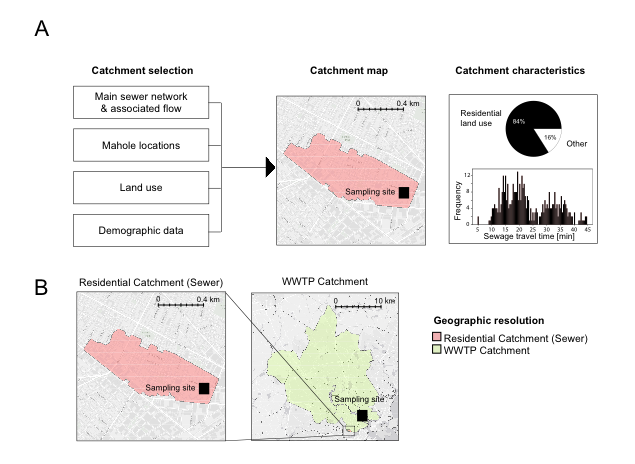
\includegraphics[width=\textwidth]{{24hr/figures/fig1_catchment_selection.png}}
    \caption{Definition and identification of residential catchments. (A). Integrating data from sewage network and flow, manhole locations, land usage, and demographic data allows for the selction of carefully curated residential manholes. (B) Upstream residential catchment vs. downstream catchment.}\label{24hr:fig1}
\end{center}
\end{figure}

\begin{figure}[h]
\begin{center}
    
\includegraphics[width=\textwidth]{{24hr/figures/fig2_upstream_downstream.png}}
    \caption{Upstream samples find more human-derived metabolites and bacteria. (A) Abundance of metabolite features in upstream vs. downstream sample (left) and volcano plot showing fold change vs. p-value (right). (B) Residential sewage sample (``Sewer'') contains more human-associated bacteria than downstream sample (``WWTP''). (C) Abundance of various confirmed human-associated metabolites in upstream vs. downstream sample.}\label{24hr:fig2}
\end{center}
\end{figure}

\begin{figure}[h]
\begin{center}
    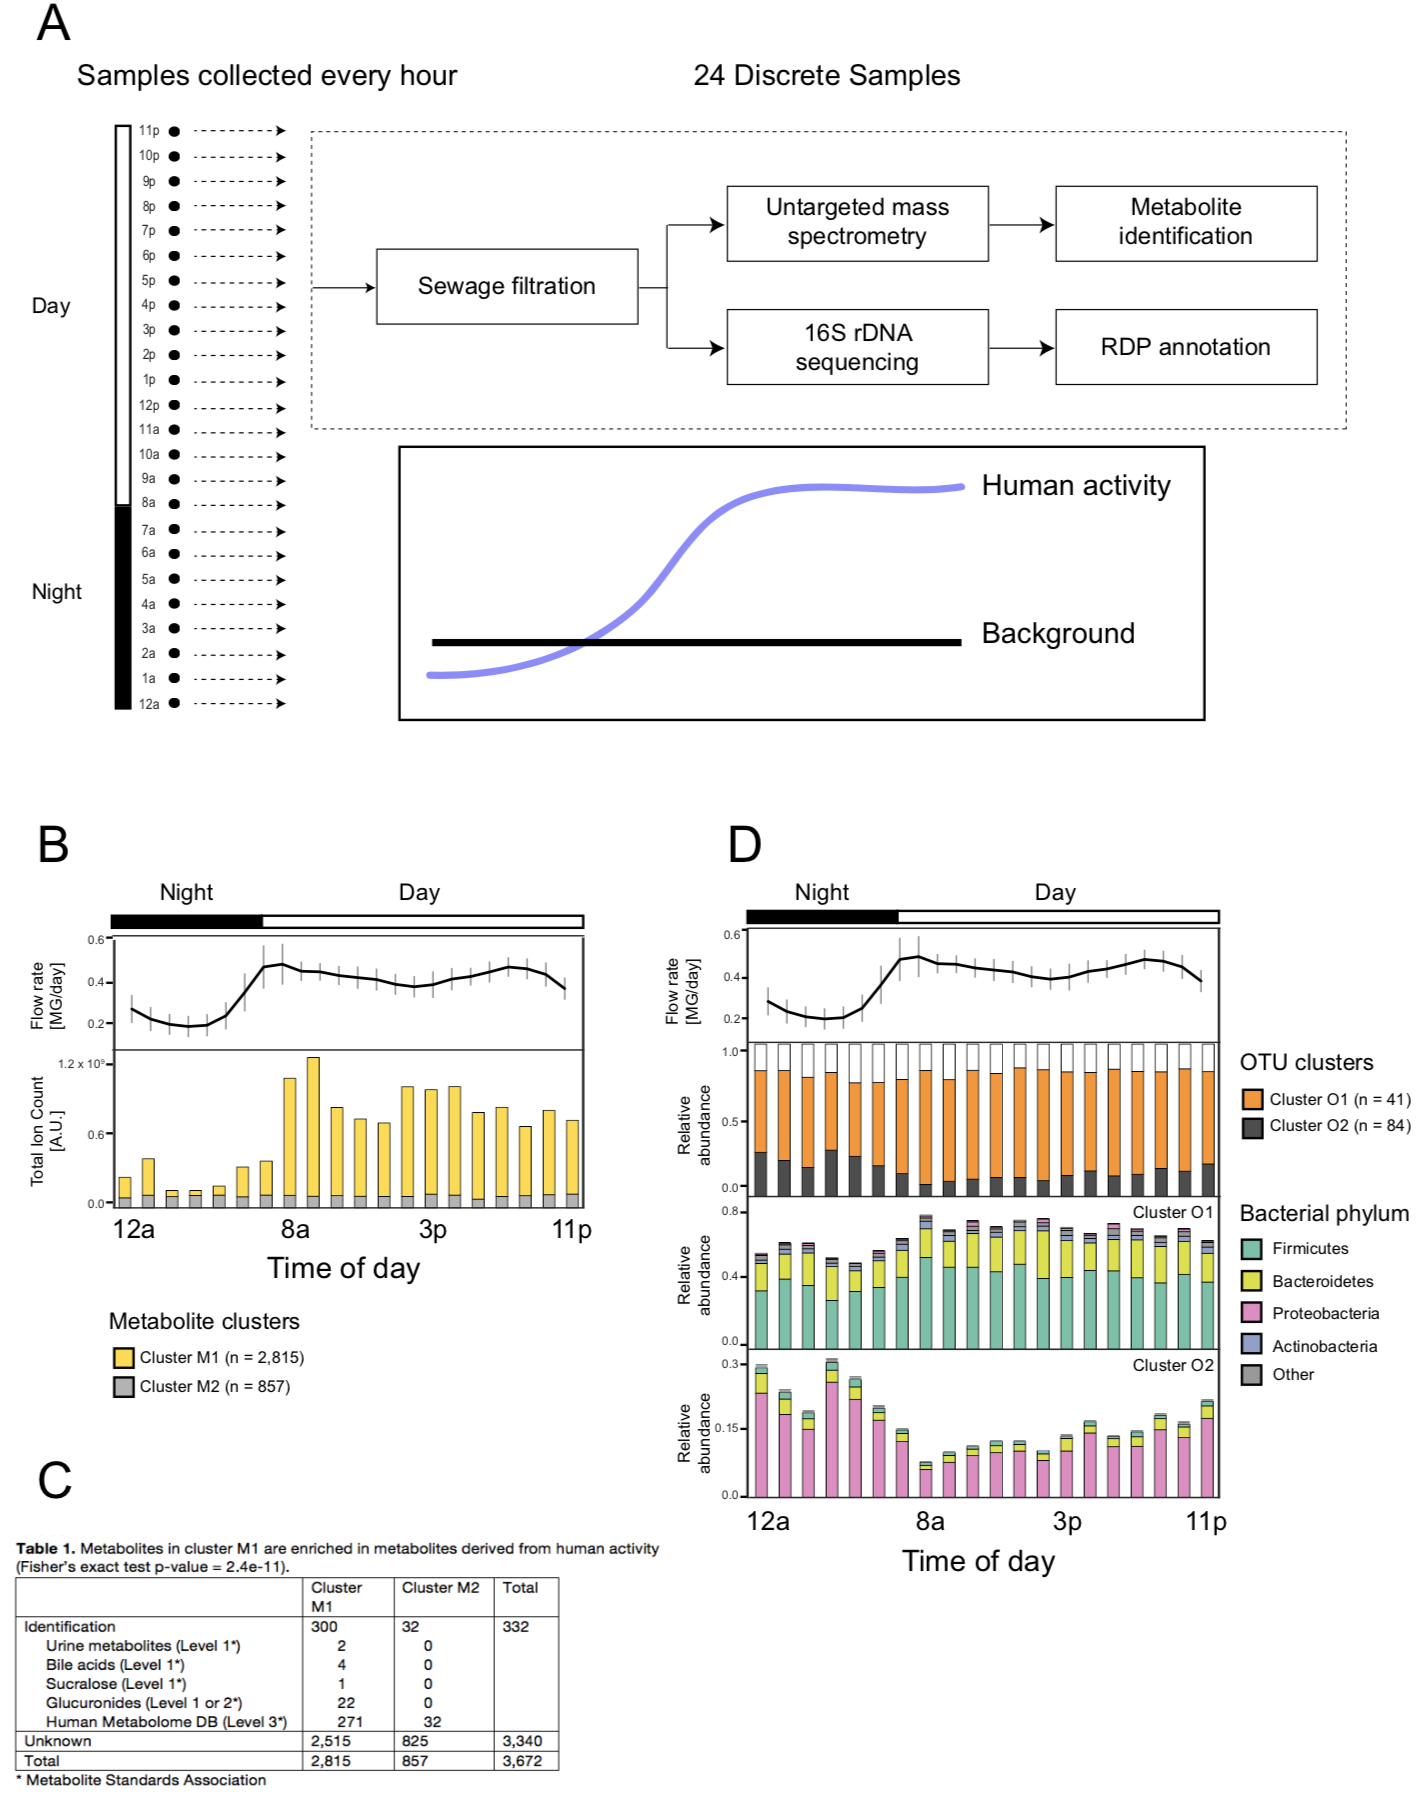
\includegraphics[width=\textwidth]{{24hr/figures/fig3_diurnal_dynamics.png}}
    \caption{Human and environmental compartments reflect human diurnal dynamics. (A) Sampling campaign and schematic of expected human activity. (B) \textit{Top}: average flow rate in residential manhole. \textit{Bottom}: total ion count of M1 and M2 metabolite clusters. (C) Number of human-associated metabolites confirmed in M1 vs. M2 clusters. (D) \textit{From top}: Average flow rate in residential manhole; relative abundance of two OTU clusters, O1 and O2; phylum-level taxonomic composition of bacterial cluster O1; phylum-level taxonomic composition of bacterial cluster O2.}\label{24hr:fig3}
\end{center}
\end{figure}

\begin{figure}[h]
\begin{center}
    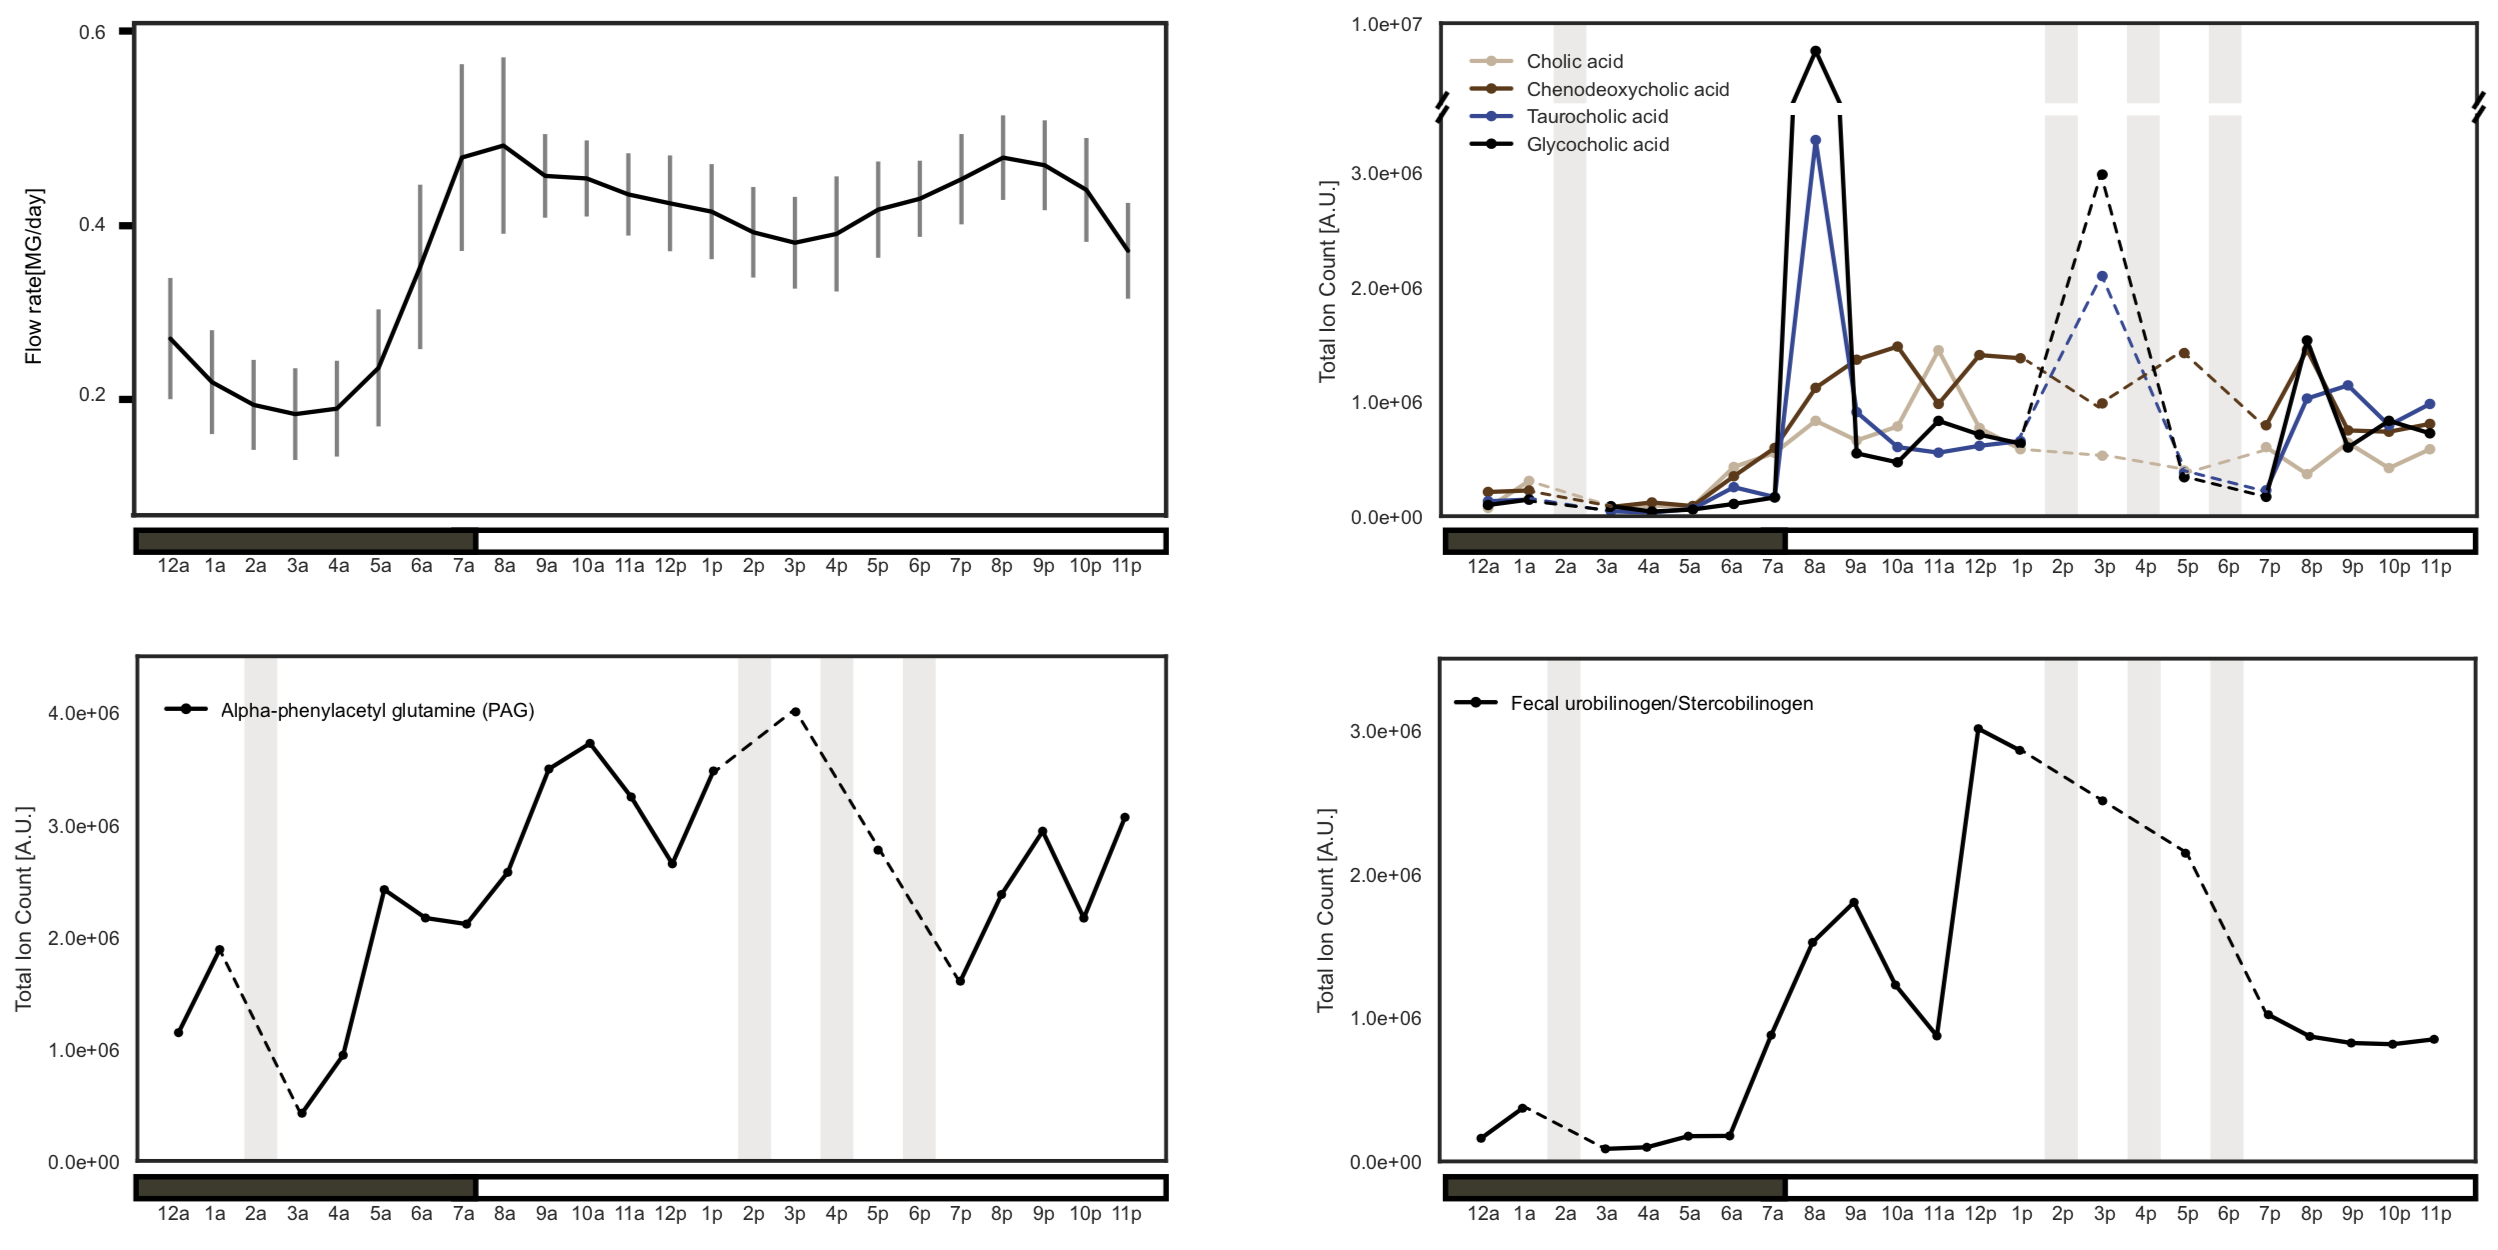
\includegraphics[width=\textwidth]{{24hr/figures/fig4_urine_fecal_markers.png}}
    \caption{Confirmed urinary and fecal biomarkers reflect human activity and behavior. (Top left) Average flow rate in residential manhole. (Bottom left) Total ion count of alpha-phenylacetylglutamine (PAG), a confirmed human urinary marker. (Top right) Total ion count of confirmed bile acids, human fecal markers. (Bottom right) Total ion count of urobilinogen, a confirmed human fecal marker. }\label{24hr:fig4}
\end{center}
\end{figure}

\begin{figure}[h]
\begin{center}
    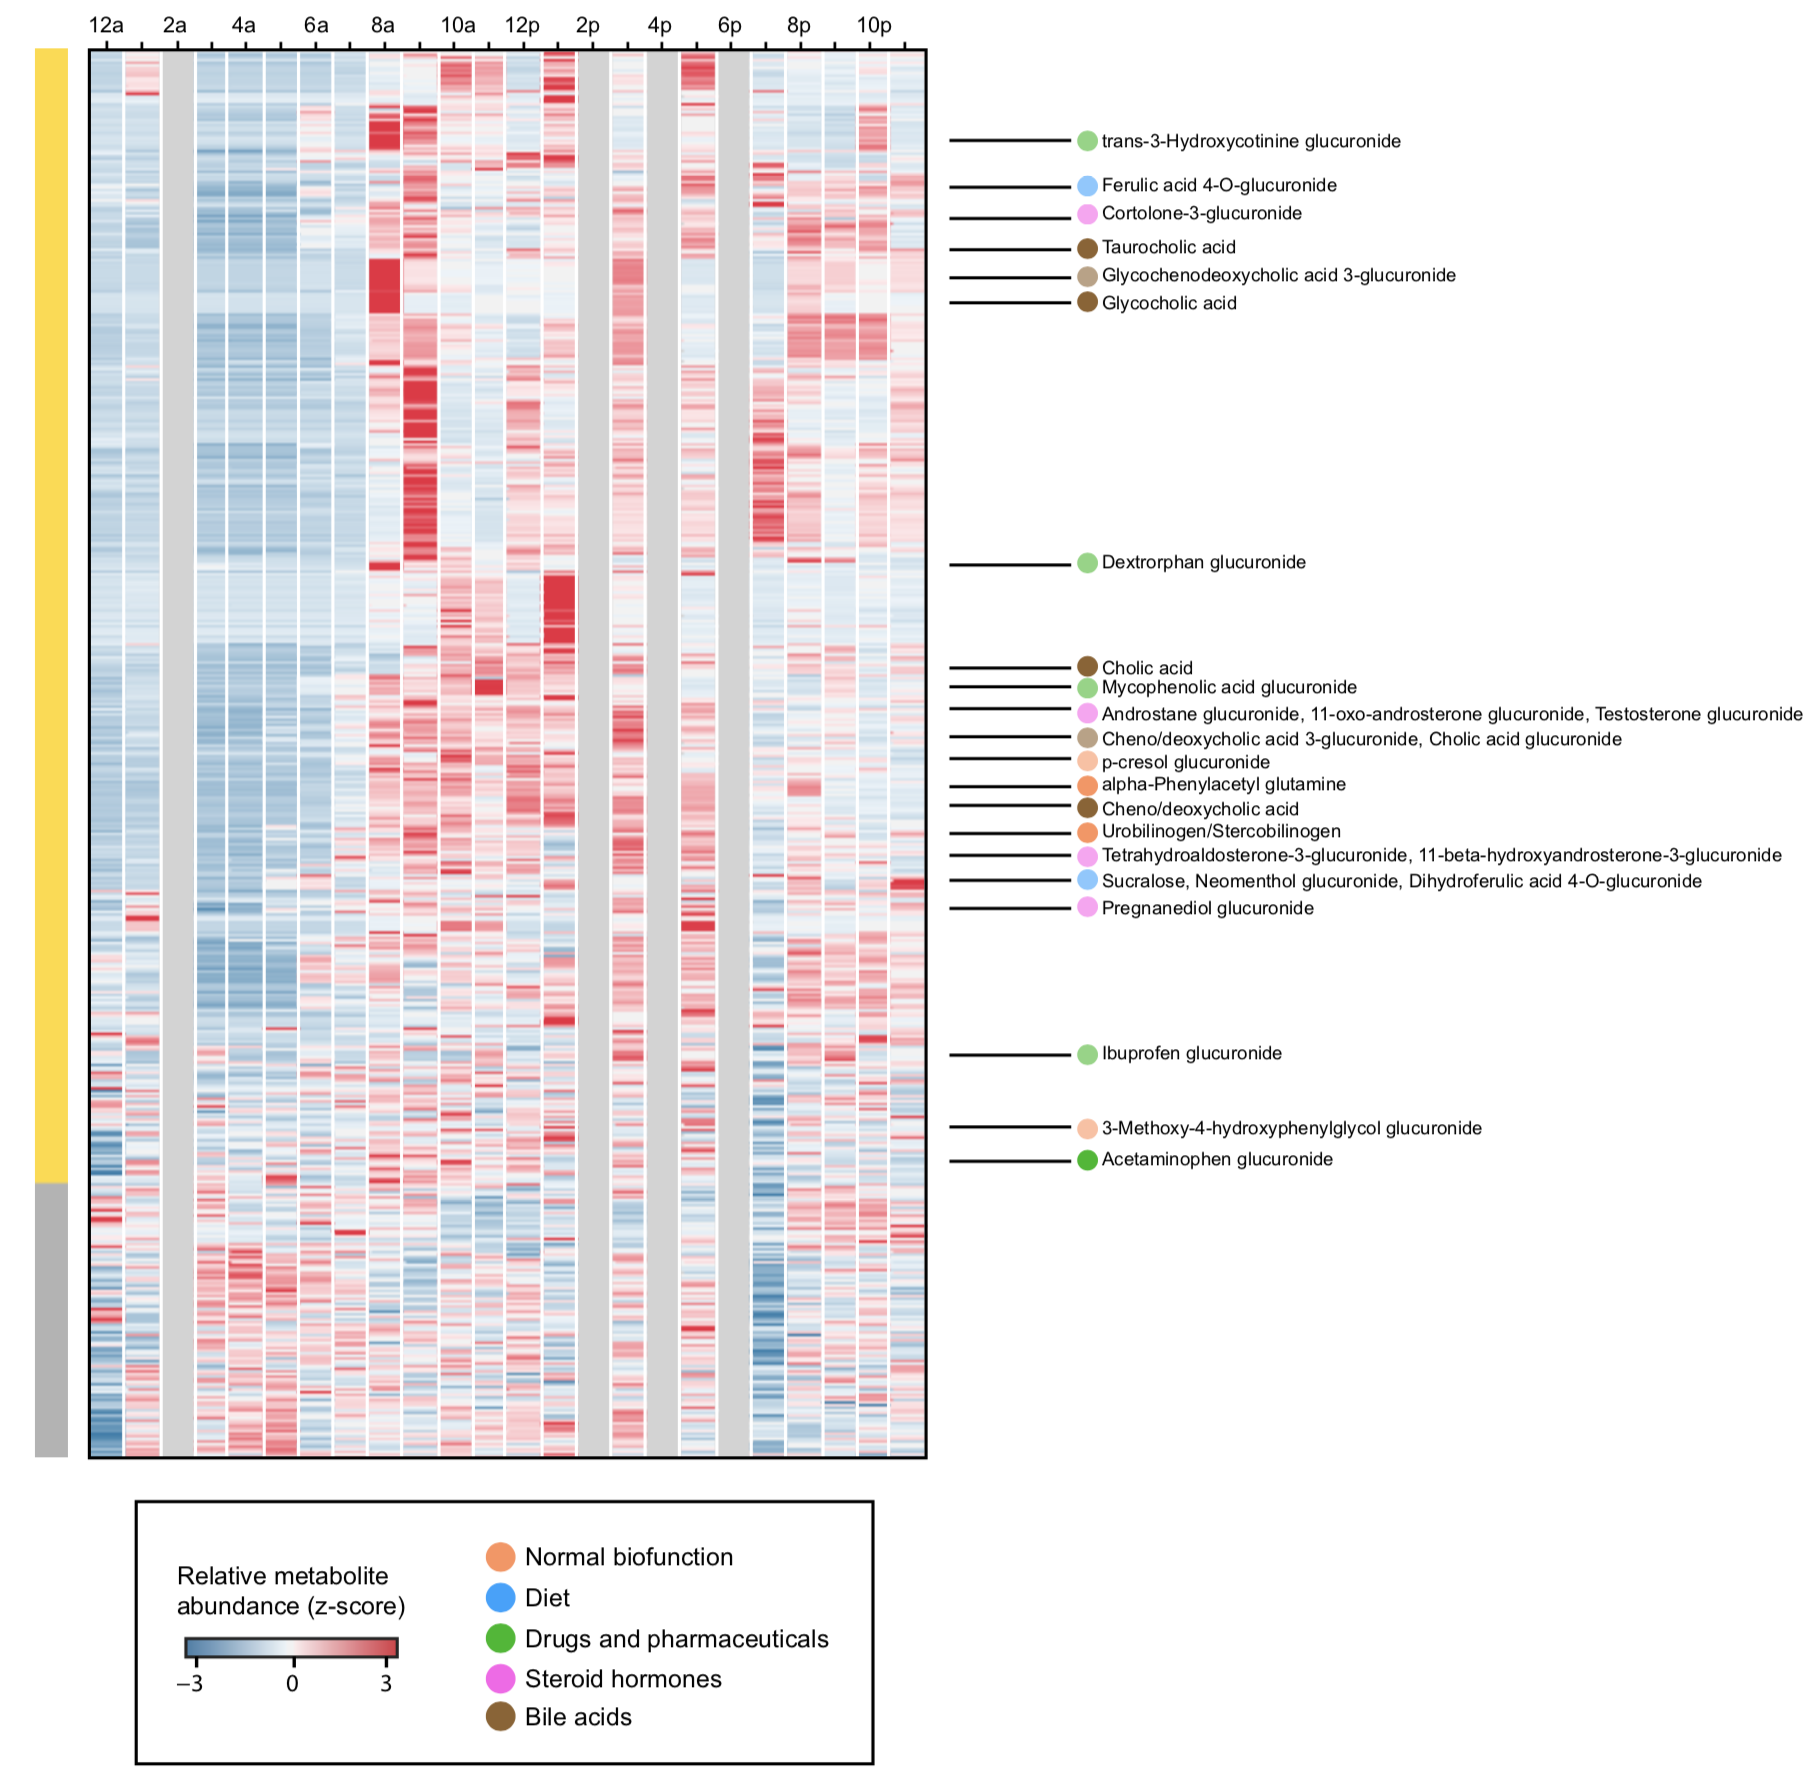
\includegraphics[width=\textwidth]{{24hr/figures/fig5_mining_big_data.png}}
    \caption{Mining untargeted data suggests identification of human health, behavioral, and lifestyle biomarkers. Heatmap of metabolite feature abundance over 24-hour samplings, with putatively identified metabolites labeled. Metabolites labeled with opaque circles were confirmed with analytical standards or MS2 matching. Labels with transparent circles were identified via mass-matching neutral mass with HMDB metabolites.}\label{24hr:fig5}
\end{center}
\end{figure}

\begin{singlespace}
\bibliographystyle{unsrtnat}
\bibliography{24hr/24hr_refs.bib}
\end{singlespace}
